\documentclass[11pt,a4paper]{article}

\usepackage[utf8]{inputenc}
\usepackage{src/classeRapport}
\usepackage{listingsutf8}
\usepackage{xcolor}
\usepackage{tabularx}
\usepackage{flafter}
\usepackage{float}
\usepackage{placeins}

\author{RJ-MH}

\setlength{\headheight}{28pt}

\lstset{
    breaklines=true,
    frame=single,
    keepspaces=true,
    numbers=left,
    moredelim = [s][\color{purple}]{/*}{*/},
    inputencoding = utf8,  % Input encoding
    extendedchars = true,  % Extended ASCII
    literate      =        % Support additional characters
      {á}{{\'a}}1  {é}{{\'e}}1  {í}{{\'i}}1 {ó}{{\'o}}1  {ú}{{\'u}}1
      {Á}{{\'A}}1  {É}{{\'E}}1  {Í}{{\'I}}1 {Ó}{{\'O}}1  {Ú}{{\'U}}1
      {à}{{\`a}}1  {è}{{\`e}}1  {ì}{{\`i}}1 {ò}{{\`o}}1  {ù}{{\`u}}1
      {À}{{\`A}}1  {È}{{\'E}}1  {Ì}{{\`I}}1 {Ò}{{\`O}}1  {Ù}{{\`U}}1
      {ä}{{\"a}}1  {ë}{{\"e}}1  {ï}{{\"i}}1 {ö}{{\"o}}1  {ü}{{\"u}}1
      {Ä}{{\"A}}1  {Ë}{{\"E}}1  {Ï}{{\"I}}1 {Ö}{{\"O}}1  {Ü}{{\"U}}1
      {â}{{\^a}}1  {ê}{{\^e}}1  {î}{{\^i}}1 {ô}{{\^o}}1  {û}{{\^u}}1
      {Â}{{\^A}}1  {Ê}{{\^E}}1  {Î}{{\^I}}1 {Ô}{{\^O}}1  {Û}{{\^U}}1
      {œ}{{\oe}}1  {Œ}{{\OE}}1  {æ}{{\ae}}1 {Æ}{{\AE}}1  {ß}{{\ss}}1
      {ç}{{\c c}}1 {Ç}{{\c C}}1 {ø}{{\o}}1  {Ø}{{\O}}1   {å}{{\r a}}1
      {Å}{{\r A}}1 {ã}{{\~a}}1  {õ}{{\~o}}1 {Ã}{{\~A}}1  {Õ}{{\~O}}1
      {ñ}{{\~n}}1  {Ñ}{{\~N}}1  {¿}{{?`}}1  {¡}{{!`}}1
      {°}{{\textdegree}}1 {º}{{\textordmasculine}}1 {ª}{{\textordfeminine}}1
      % ¿ and ¡ are not correctly displayed if inconsolata font is used
      % together with the lstlisting environment. Consider typing code in
      % external files and using \lstinputlisting to display them instead.
  }



\begin{document}

\PageDeGarde
{couverture.jpeg} % image sur la page de garde
{Projet TW2} % titre principal
{Idle Game :} % sous-titre
{
Ambre \textsc{De crescenzo}\\
Nils \textsc{Etien}\\
Maxime \textsc{Huyenh}\\% noms
Ryan \textsc{Juteau}\\

}
{TW2 - ITI4 - 2022} % bas de page

\Page{INSALogo}{rien.png} % logo de bas de page (en bas a droite)


\tableofcontents

\clearpage


\section{Introduction}

  \subsection{Présentation du projet}

    L'objectif de ce projet est de développer un Idle game et de se familiariser avec les technologies vues durant le cours de Technologie Web 2. Ce sera un jeu de Gacha. Ce type de jeu est assez addictif et se base sur l'obtention aléatoire de loot ce qui pousse les joueurs à continuer afin d'en débloquer toujours plus. Nous allons notamment utiliser Node.js et Express.js par exemple, et la base de données sera en SQLite.


\clearpage

\section{Specifications}

\subsection{Spécifications fonctionnelles}

    \subsubsection{Fonctionnalités obligatoires}

        \begin{itemize}
            \item Création de compte : Le joueur doit pouvoir choisir une adresse mail qui n’est pas déjà utilisée, et un mot de passe. Le mot de passe sera hashé pour plus de sécurité. Lorsque le compte est créé, l’authentification est lancée avec les données rentrées lors de la création du compte pour que le jeu commence dès la création du compte (sans avoir à s’authentifier après avoir créé son compte).

            \item Authentification : Une personne qui possède un compte peut se connecter avec son pseudo et son mot de passe, ce qui charge la sauvegarde du joueur et lance le jeu avec la sauvegarde du joueur.


            \item Sauvegarde : Quand le joueur quitte la page, il est déconnecté et la sauvegarde est stockée dans une base de données contenant l’adresse mail du joueur, le mot de passe du joueur, ses améliorations, ses personnages, son argent/ses diamants, ses armes (optionnel), les niveaux de ses armes (optionnel).

            \item  Détails sur le jeu : Héros

            \begin{itemize}
                \item Le premier héros est donné de base, niveau 1.

                \item Les héros créent des golds chaque seconde (golds/s)

                \item Ces golds servent à monter de niveau les héros (en cliquant sur un bouton) et donc à augmenter les golds/s obtenus par ces héros (multiplicatif par rapport à ses valeurs de golds/s (voir ci-après)).

                \item Le coût des niveaux augmente non linéairement. Tous les 100 niveaux, les golds/s sont doublés et tous les 10 niveaux, le héros gagne 1 diamant/s supplémentaire

                \item Les héros les plus rares sont plus difficiles à monter de niveau, mais donnent plus de golds/s et de diamants/s que les personnages moins rares.

                \item  Ces diamants servent à invoquer des héros. Pour 160 diamants, on peut invoquer un nouveau héros (héros commun : 94.3\%, rare : 5.1\%, légendaire : 0.6\%) ; 1 héros rare garanti tous les 10 voeux (si aucun rare obtenu dans les 9 premiers voeux) ; 1 héros légendaire garanti tous les 90 voeux(si aucun légendaire obtenu dans les 90 derniers voeux)

                \item Si on obtient un doublon de héros commun, on obtient rien.

                \item Si on obtient un doublon de héros rare, on obtient 160 diamants.

                \item Si on obtient un doublon de héros légendaire, on obtient 1600 diamants.

                \item Le jeu terminé lorsque tous les héros sont obtenus et niveau maximum (1000?), et toutes les armes ont été obtenues et niveau maximum(100?) (optionnel).
            \end{itemize}



        \end{itemize}



    \subsubsection{Fonctionnalités optionnelles}


        \begin{itemize}
            \item Guide” où le joueur peut voir des détails sur les héros, les armes (voir ci-après), les invocations, etc etc…

            \item Edition d’un compte : L’utilisateur peut changer son mot de passe et son adresse mail dans le menu des Options du jeu (après connexion).

            \item Cliquer : L’utilisateur peut cliquer sur un ennemi pour obtenir des golds (change en fonction des améliorations des héros) (20\% des golds/s et diamant/s totaux).

            \item Si on a créé une sauvegarde : si on quitte le jeu et qu’on se reconnecte X heures plus tard, on gagne Y golds et Z diamants en fonction du temps passé hors jeu (8\% de ce qui aurait été gagné en laissant le jeu ouvert).

            \item Le pseudo du joueur est demandé au commencement d’une nouvelle partie, puis, après avoir rentré un pseudo, le joueur choisit un premier héros (parmi une liste de héros). Ce premier héros a pour nom le pseudo rentré par le joueur.

            \item Le joueur a le choix entre 3 sauvegardes, et peut cloner/supprimer ses sauvegardes. S’il sélectionne une sauvegarde vide, cela crée/commence une nouvelle sauvegarde. On voit le pseudo du joueur sur la sauvegarde (voir proposition ci-dessus), et un symbole (une couronne?) si le joueur a “terminé” le jeu(voir dernière proposition de la catégorie “Fonctionnalités obligatoires”).

            \item Musique et effets sonores.

            \item Dans le menu des Options : options pour régler le volume de la musique et des effets sonores. Affichage des crédits. Option pour supprimer la sauvegarde (si on a une seule sauvegarde).

            \item Cycle jour/nuit (Jour : normal, Nuit : -golds/s, +diamants/s)

            \item Détails sur le jeu : Armes

            \begin{itemize}

                \item Toutes les minutes, le joueur a 15\% de chance d’obtenir une arme (ratios de raretés identiques à ceux des héros).

                \item Une arme peut être équipée à un héros et un seul (si on équipe une arme déjà équipée, l’arme change de propriétaire).

                \item Une arme augmente les statistiques (golds/s et diamants/s) de base du héros qui équipe cette arme (appliqué avant le coefficient multiplicatif des niveaux).

                \item On peut aussi invoquer des armes pour 160 diamants, avec le même système que les héros (doublons inclus).

                \item Jeu sauvegardé toutes les 5 minutes(après la possible obtention de l’arme qui arrive à chaque minute) en plus de la sauvegarde quand on quitte le jeu.

                \item Chaque héros a un type d’arme de prédilection (épée, faux, lance, bâton, arc, poings, griffes) etc etc… : si le héros est équipé du type d’arme en question, le bonus de l’arme est doublé.

                \item Certaines armes peuvent donner des bonus supplémentaires (golds/s, diamants/s) si un héros spécifique l’équipe (différent du type d’arme de prédilection, se combine avec le type d’arme de prédilection)

                \item Les armes gagnent de l’expérience en fonction du nombre de golds/s du héros qui équipe l’arme. Cette expérience fait monter l’arme de niveau et augmente les statistiques de l’arme. Les niveaux sont plus difficiles à monter pour les armes les plus rares.

            \end{itemize}



        \end{itemize}


\clearpage
\subsection{Specifications d'interfaces}

    \subsubsection{Interfaces obligatoires}

        \begin{figure}[ht!]
            \centering
                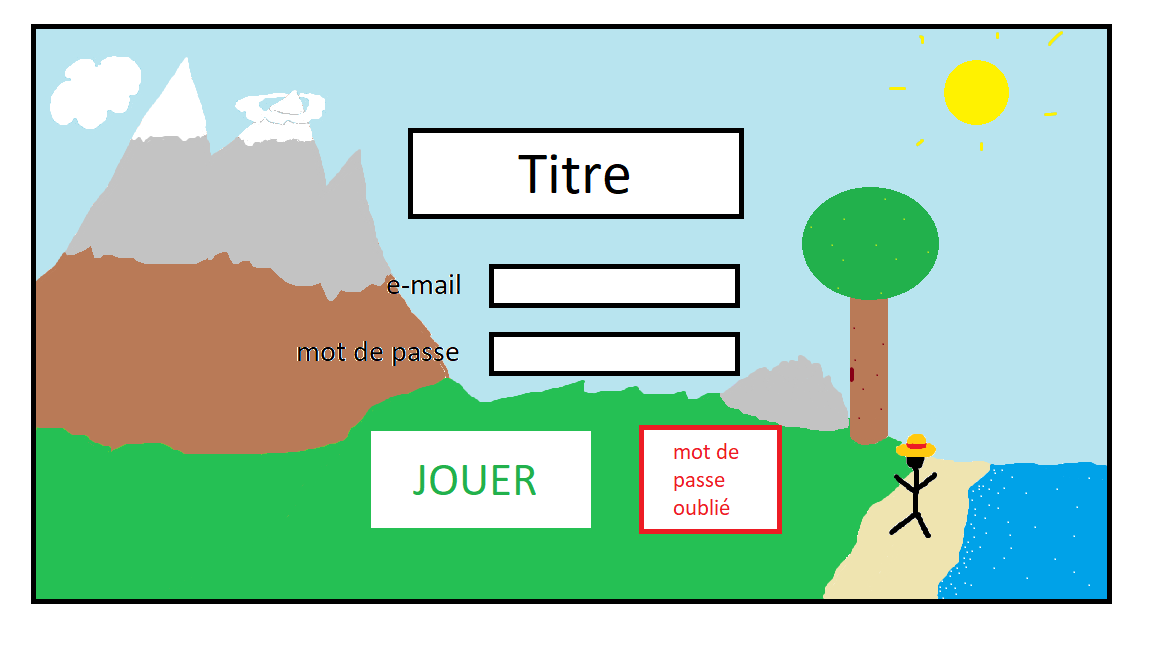
\includegraphics[width=0.8\textwidth]{images/EcranTitre.png}
            \caption{Interface pour la connexion/création de compte}
        \end{figure}


        \begin{figure}[ht!]
            \centering
                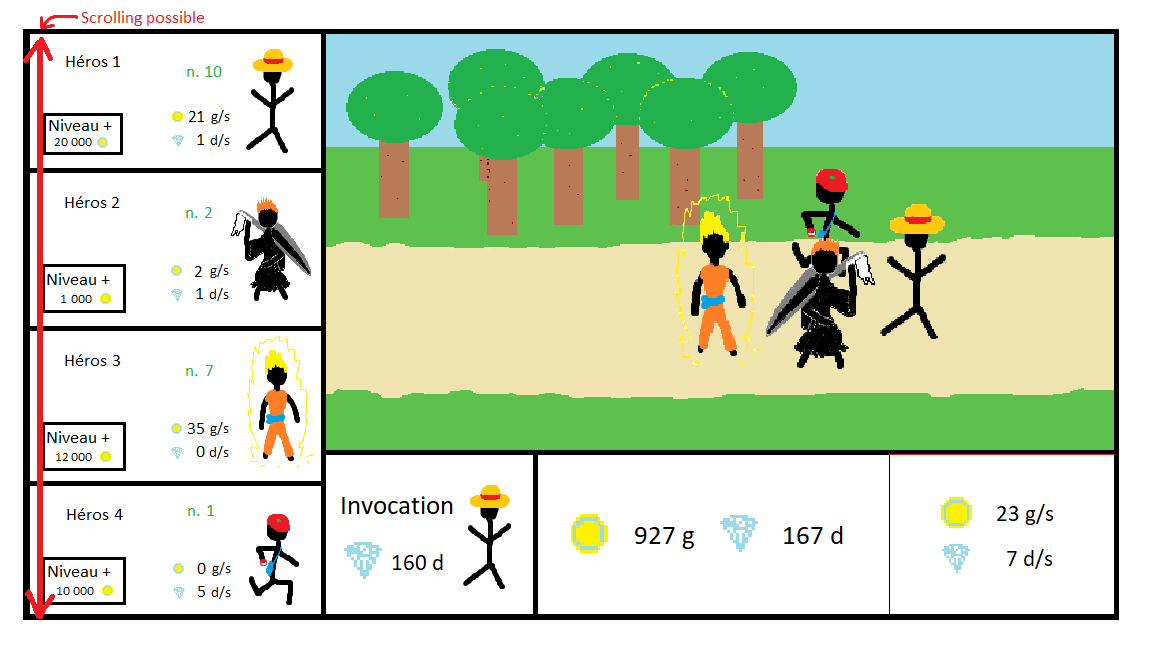
\includegraphics[width=0.8\textwidth]{images/TWJeuHUDSansOptions.png}
            \caption{Interface du jeu}
        \end{figure}

        \newpage

    \subsubsection{Interfaces facultatives}

        \begin{figure}[ht!]
            \centering
                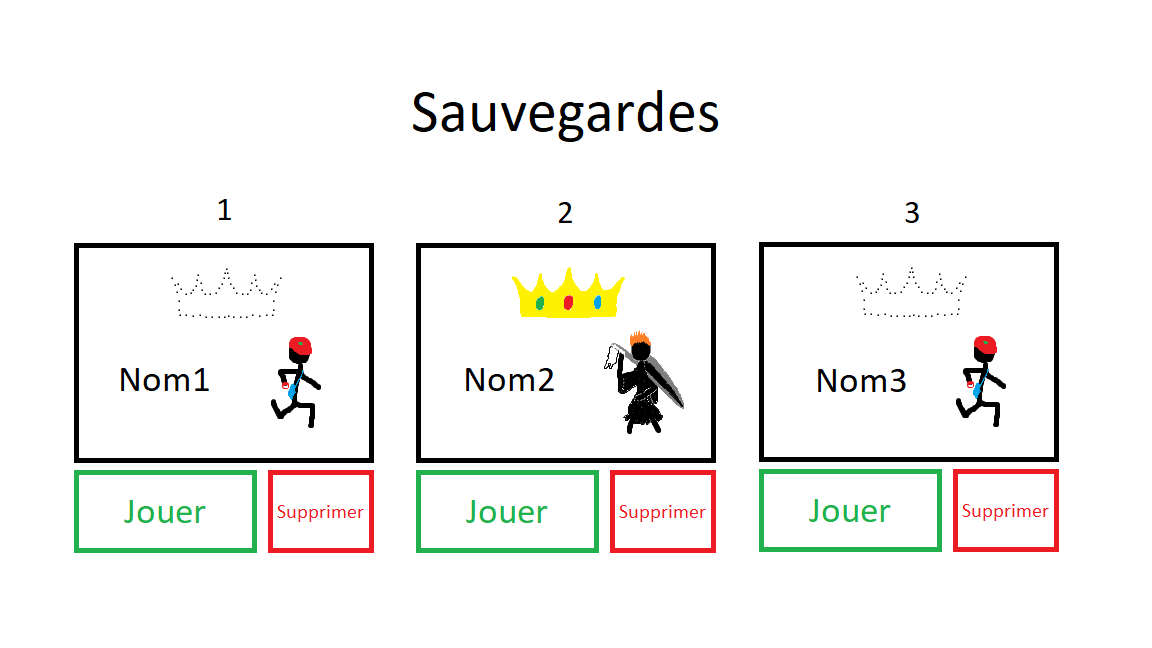
\includegraphics[width=0.8\textwidth]{images/ChoixSauvegarde.png}
            \caption{Interface pour la sélection de sauvegarde}
        \end{figure}

        \begin{figure}[ht!]
            \centering
                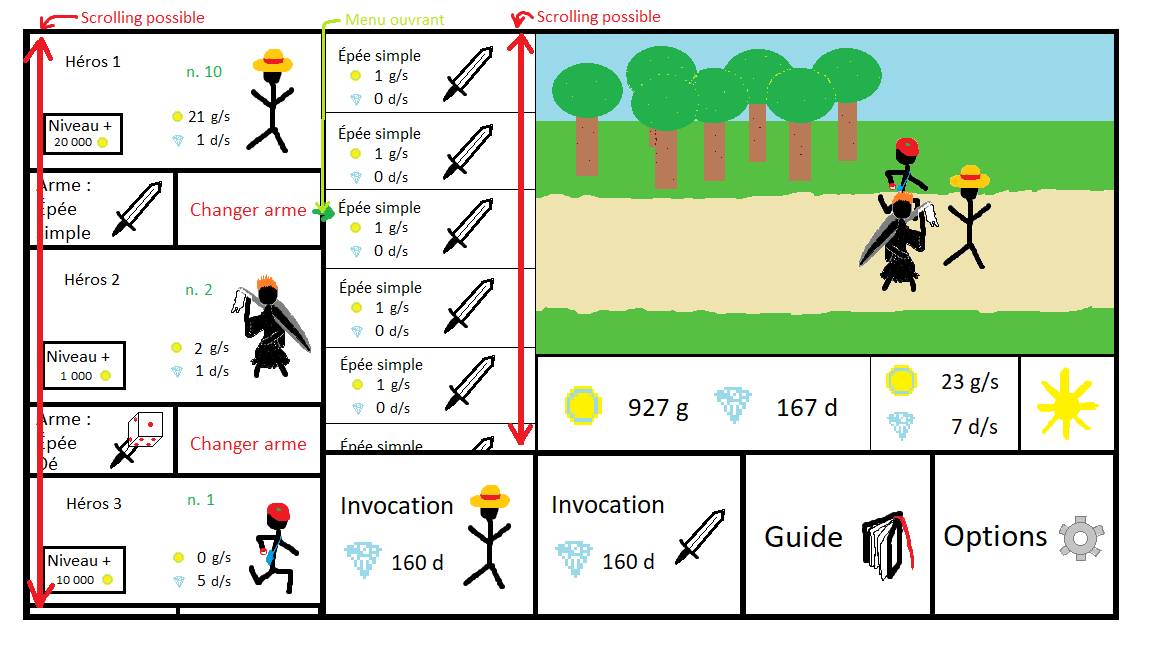
\includegraphics[width=0.8\textwidth]{images/TWJeuHUD.png}
            \caption{Interface du jeu avec les fonctionnalités optionnelles}
        \end{figure}


\clearpage
\subsection{Specifications opérationnelles}


\clearpage
\subsection{Specifications des rôles}

    \begin{figure}[h!]
        \centering
            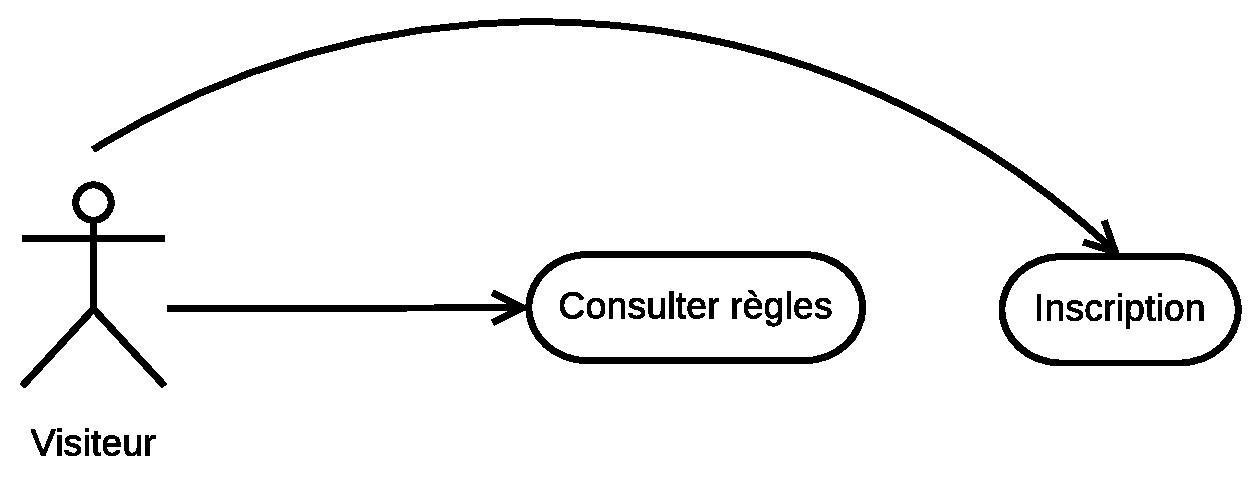
\includegraphics[width=0.8\textwidth]{images/utilisation1.eps}
        \caption{Diagramme à l'écran titre pour un visiteur}
    \end{figure}

    \begin{figure}[ht!]
        \centering
            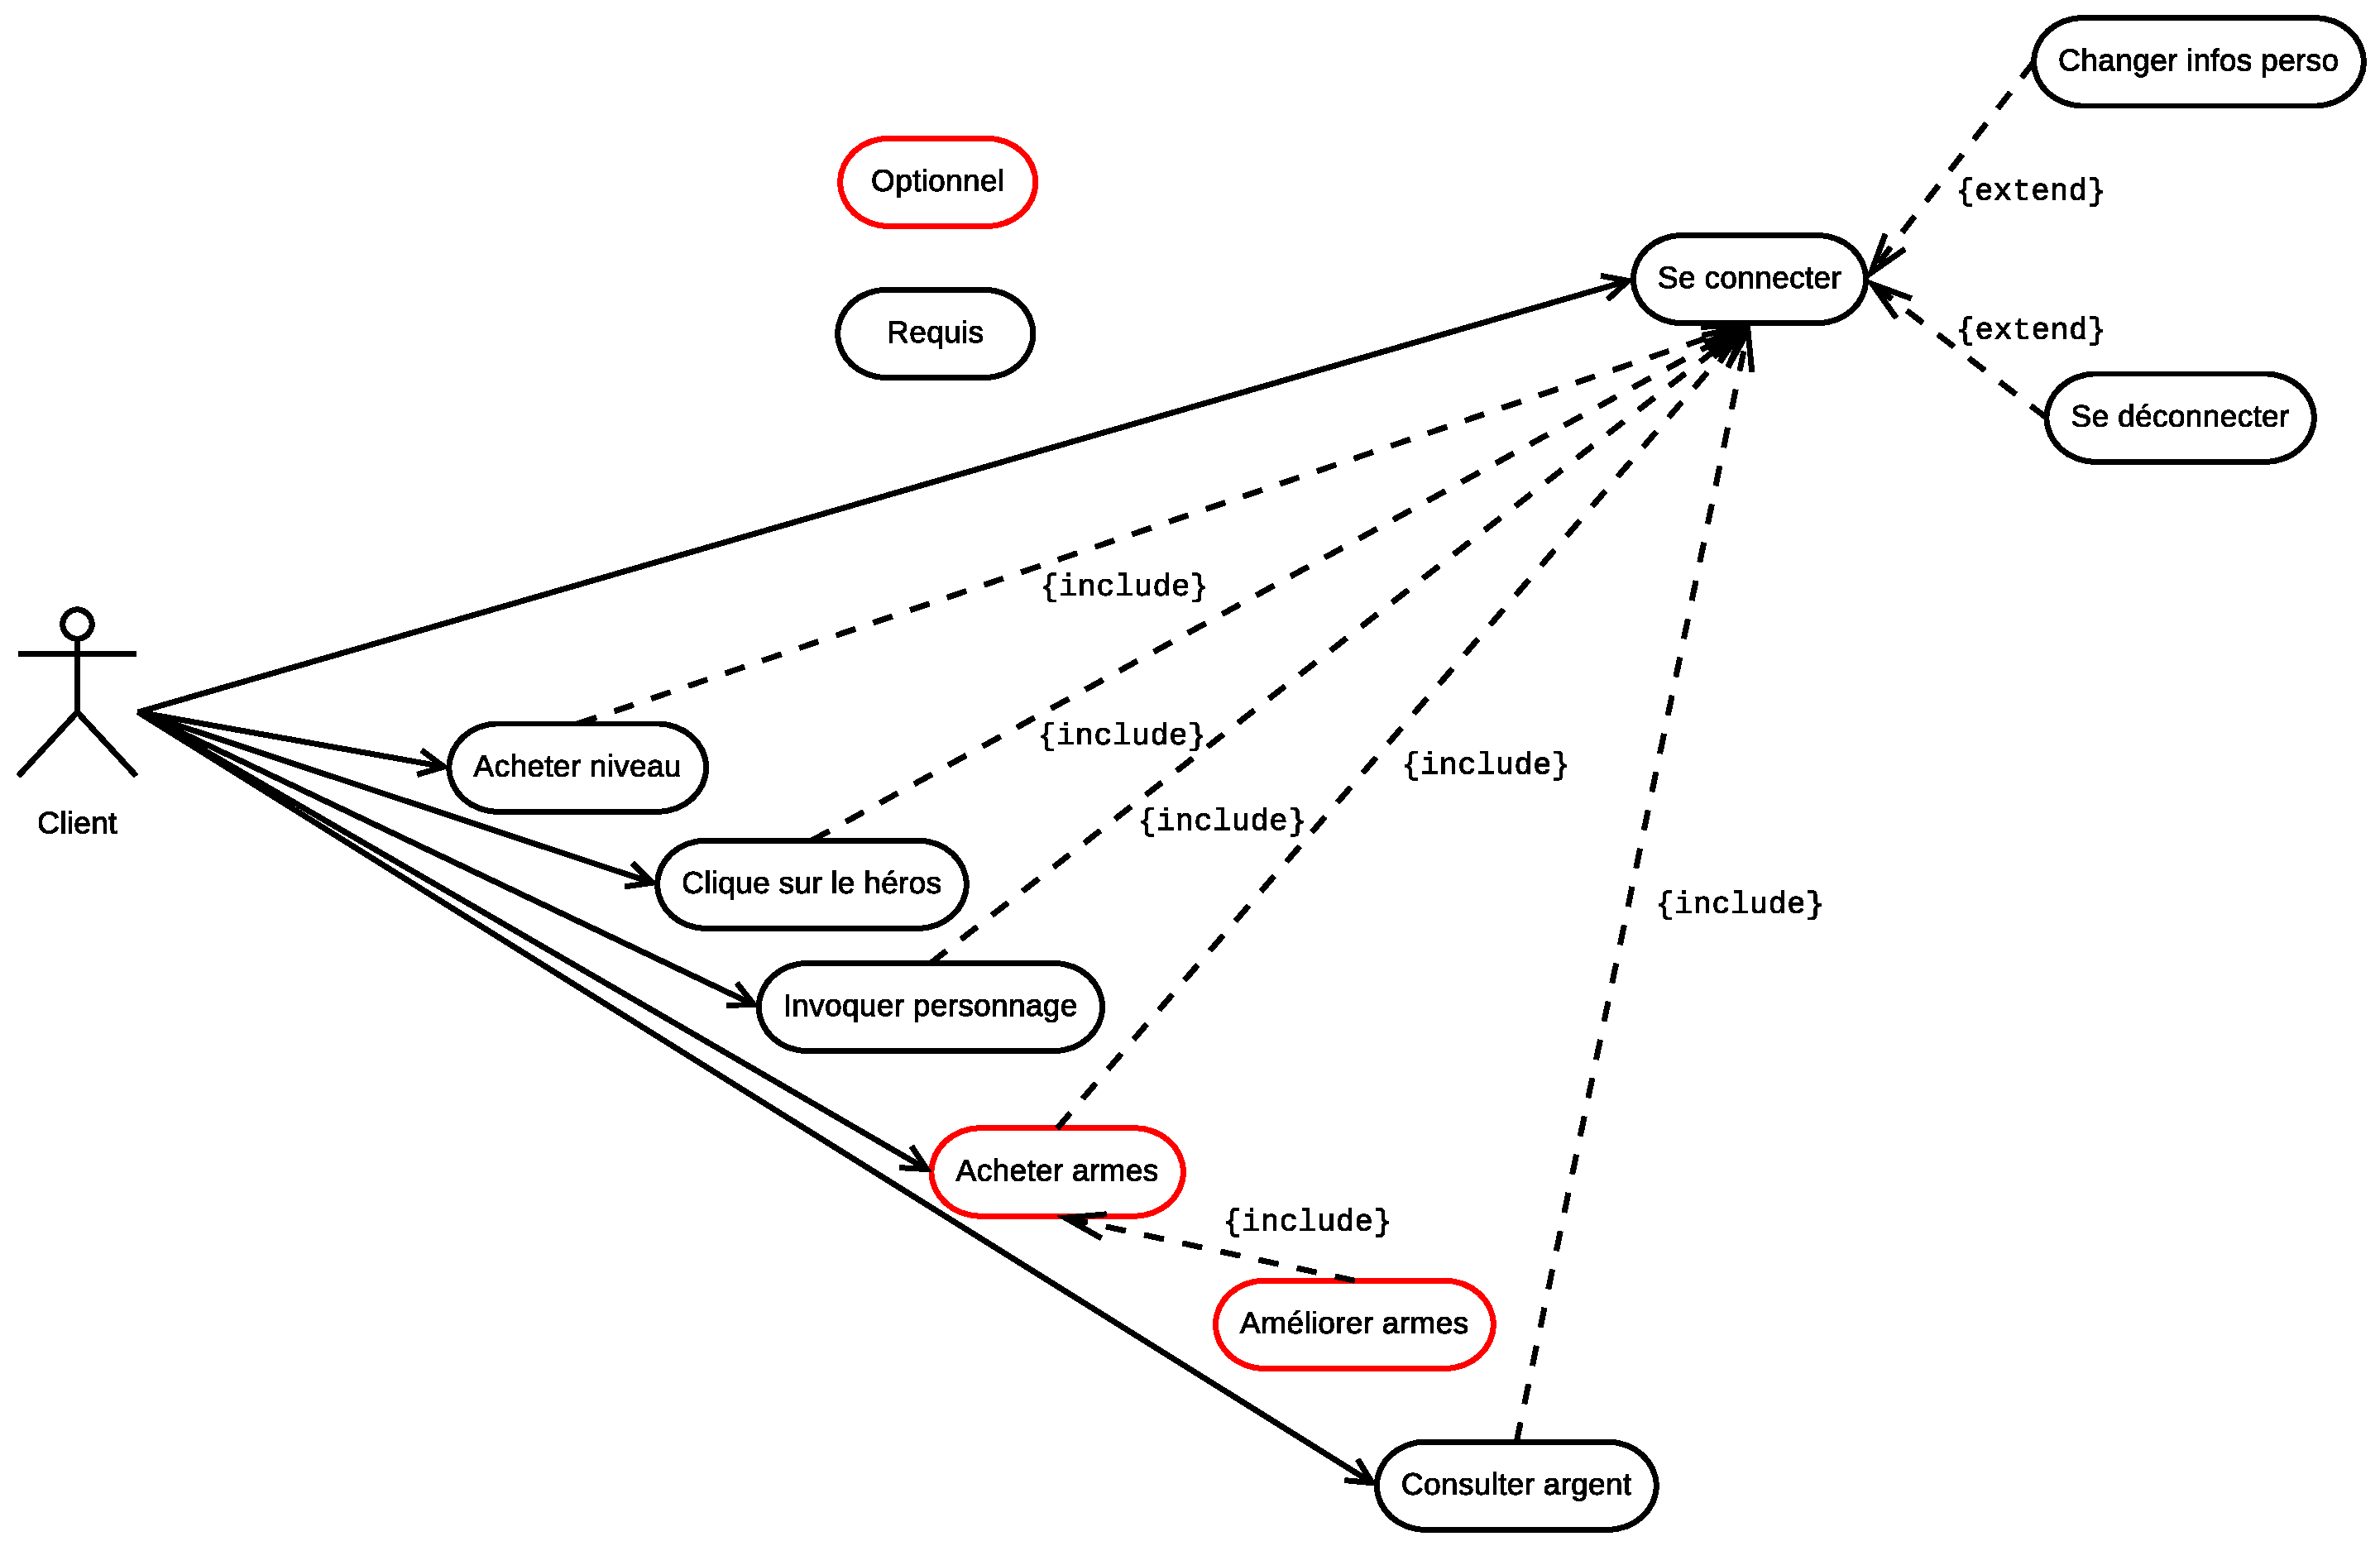
\includegraphics[width=1\textwidth]{images/utilisation2.eps}
        \caption{Diagramme pendant le jeu pour un utilisateur}
    \end{figure}

    \newpage

    \begin{figure}[ht!]
        \centering
            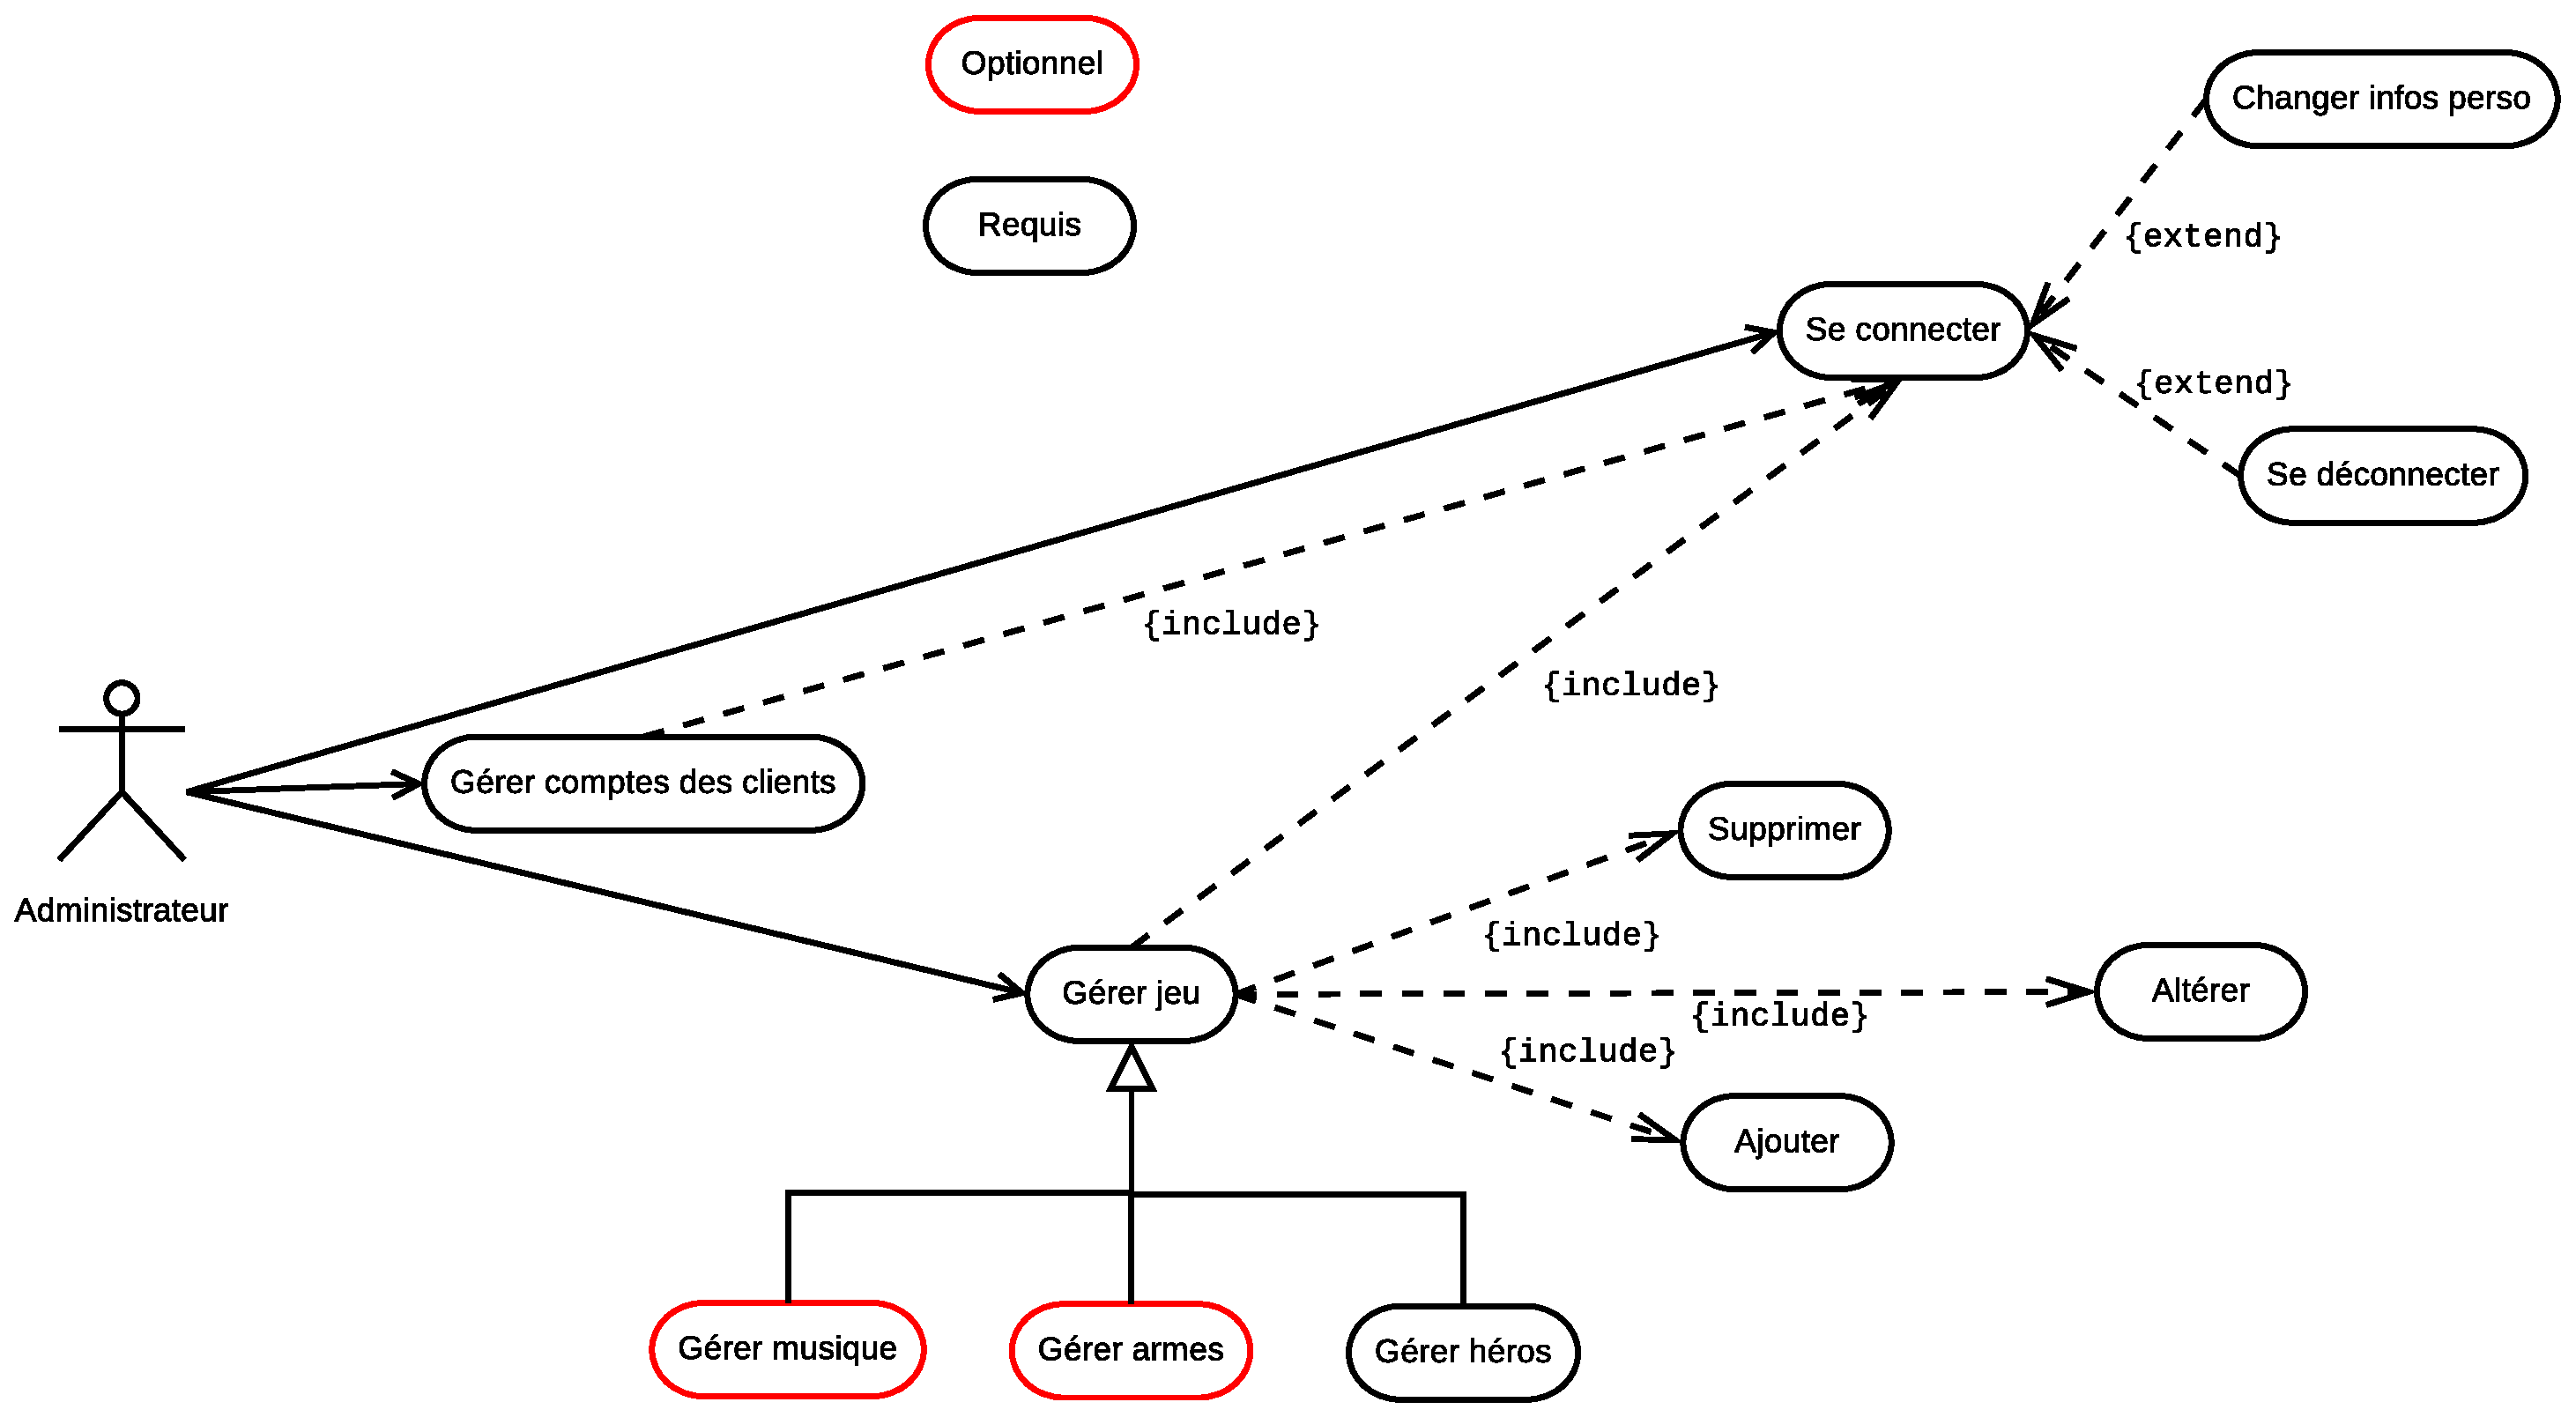
\includegraphics[width=1\textwidth]{images/utilisation3.eps}
        \caption{Diagramme pour un administrateur}
    \end{figure}


\clearpage

\section{Conception}

\subsection{Diagramme de séquence}


\clearpage
\subsection{Diagramme de navigation}


\clearpage
\subsection{Diagrammes de classes}

    \begin{figure}[ht!]
        \centering
            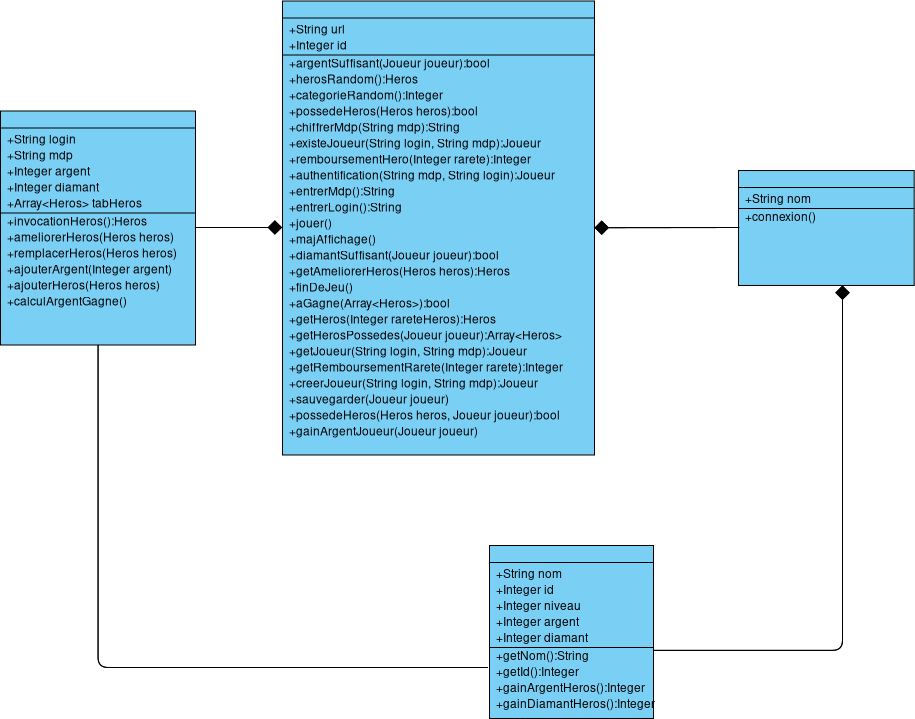
\includegraphics[width=1\textwidth]{images/Diagramme_de_classe_TW2_V4.png}
        \caption{Diagramme de navigation}
    \end{figure}


\clearpage
\subsection{Représentation logique de la base de données}


\end{document}
